\problemname{Letter dice}

Klara has $N$ dices with letters written on them.
Each die has a letter on each of its $K$ sides.
By throwing the dice and rearranging them in some arbitrary order, you can make construct a word with $N$ letters.

Write a program to count the number of valid words that can be constructed using Klara's dice.
You will get a wordlist, that contains all the $M$ valid $N$-letter words.

\begin{figure}[ht!]
\centering
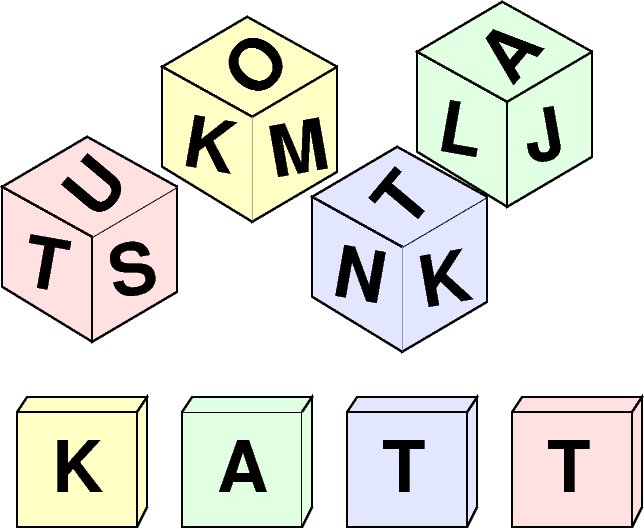
\includegraphics[width=0.6\textwidth]{tarningar.png}
\caption{An illustration of the first example. Since $K = 3$, each die has three sides. You can also write \texttt{STOL} and \texttt{MASK}, but not \texttt{NATT} or \texttt{KOST}.}
\label{overflow}
\end{figure}

\section*{Input}

The first line of input contains three space-separated integers $N$, $K$ and $M$.

The next $N$ lines each describe a die. Line $i$ will contain $K$ letters, the letters on the sides of the $i$:th die.

Finally, there will be $M$ lines, the valid words. Each line will contain an $N$-letter word.

All words will only capital letters \texttt{A-Z}.

No letter will appear on more than one side of a die.

\section*{Output}
Your program should print a single integer: the number of valid words that can be written.


\section*{Scoring}
Your solution will be tested on a number of test case groups. To get points for a group
you have to solve all the test cases in that group.

\begin{tabular}{| l | l | l | l |}
\hline
Group & Points & Limits & Other \\ \hline
	1     & 9          & $K = 2, N \le 4, M \le 100$ \\ \hline
	2     & 9          & $K \le 6, N \le 5, M \le 100$ \\ \hline
	3     & 12         & $K \le 20, N \le 6, M \le 1000$ \\ \hline
	4     & 14         & $K \le 15, N \le 6, M \le 10\,000$ \\ \hline
	5     & 21         & $K \le 20, N \le 6, M \le 100\,000$ \\ \hline
	6     & 35         & $K \le 10, N \le 13, M \le 500$ \\ \hline
\end{tabular}
